\documentclass[12pt]{article}
\usepackage{fullpage}
\usepackage{amsmath, amsthm, amssymb}
\usepackage{enumerate}
\usepackage{mathtools}
\usepackage{multicol}
\usepackage{nicefrac}
\usepackage{graphicx}
\usepackage{float}
\newtheorem{lemma}{Lemma}
\newtheorem{theorem}{Theorem}
\usepackage{subcaption}

\newcommand*{\Real}{\mathbb{R}}
\newcommand*{\ord}{\mathrm{ord}}
\newcommand*{\inv}{^{-1}}

\begin{document}

\title{MATH 4320 Homework 2}
\author{Dominick Twitty}
\date{}
\maketitle

\section{Proving and Disproving Groups}
\begin{enumerate}[(a)]
\item $\Real^{\geq 0}$ with operation $a \star b = \max(a,b)$ is not a group. We have that $\max(a, 0) = \max(0, a) = a$, which means the identity element $e = 0$. However, for any $a > 0$, there is no $b$ such that $\max(a, b) = 0$. There is no inverse element, so this is not a group.

\item $\Real^\times$ with operation $a \star b = \frac{a}{b}$ is not a group. We attempt to verify associativity:
\begin{align*}
a \star (b \star c) &= (a \star b) \star c\\
\frac{a}{\nicefrac{b}{c}} &= \frac{\nicefrac{a}{b}}{c}\\
\frac{ac}{b} &\neq \frac{a}{bc}
\end{align*}

\item $\Real$ with operation $a \star b = \text{frac}(a, b) = ab - \lfloor ab \rfloor$ is not a group. We have an operation that is a function $\star : \Real \times \Real \rightarrow [0, 1)$. If $a$ is greater than 1, there is no $b$ such that $\text{frac}(a, b) = a$, as $a$ is not in the codomain of $\star$. Therefore, the group has no identity element. 

\item The cartesian product $A \times B$ where $A$ and $B$ are groups, which we call $G$, with operation $(a, b) \star (c, d) = (ab, cd)$ is a group. Because $A$ and $B$ are closed, we have that operation $\star : (A \times B) \times (A \times B) \rightarrow A \times B$, we know that $G$ is closed.

We show associativity:
\begin{align*}
(a,b) \star ((c, d) \star (e, f)) &= ((a,b) \star (c, d)) \star (e, f)\\
(a, b) \star (ce, df) &= (ac, bd) \star (e, f)\\
(ace, bdf) &= (ace, bdf)
\end{align*}

Let $e$ be the identity element of $A$ and $f$ be the identity element of $B$. We have
\begin{align*}
(e, f) \star (a, b) &= (a,b) \star (e, f)\\
(ea, fb) &= (ae, bf)\\
(a, b) &= (a, b)
\end{align*}

So $(e, f)$ is the identity element of $G$. Finally, we show inverse elements:
\begin{align*}
(a, b) \star (a^{-1}, b^{-1}) &= (a^{-1}, b^{-1}) \star (a, b)\\
(aa^{-1}, bb^{-1}) &= (a^{-1}a, b^{-1}b)\\
(e, f) &= (e, f)
\end{align*}

$G$ meets all the requirements of a group.

\end{enumerate}

\section{Finite Groups Imply Finite Order}
We have that $G$ is a finite group, and we wish to show that $\ord(a) < \infty$ for all $a$ in $G$. That is, we wish to show that there exists some finite $m > 0$ such that $a^m = e$. 

\begin{lemma}
For $a$ in finite group $G$, there exists $m \neq n$ such that $a^n = a^m$.
\end{lemma}
\begin{proof}
By the closure property of groups, we have that $a^k \in G$. By the pigeonhole principle, the list $a^1, a^2, a^3,\ldots$ must eventually repeat. If the list did not repeat, $G$ could not be closed unless $G$ were infinite. Because the list repeats, there must exist two powers that equal each other.
\end{proof}

By the previous lemma, we have for every $a$ there exists some $m < n$ with $a^m = a^n$. Then, we have that $a^{n - m} = e$. 

\section{Identity Squares Imply Abelian}
\begin{lemma}
If $G$ is a group and for all $x$ in $G$ we have $x^2 = 1$, then $G$ is abelian.
\end{lemma}
\begin{proof}
Showing that a group is abelian is equivalent to showing $xy = yx$.
\begin{align*}
xy &= yx\\
y(xy)x &= y(yx)x\\
(yx)(yx) &= (yy)(xx)\\
(yx)^2 &= y^2 x^2\\
1 &= 1
\end{align*}

\end{proof}

\pagebreak
\section{$S_n$ and $D_{2n}$ Isomorphisms}
We show that $S_3$ and the dihedral group of order 6 are isomorphic by bringing their multiplication tables to the same form. Here are the members of the dihedral group [ProofWiki]

\begin{figure}[!htb]
\centering
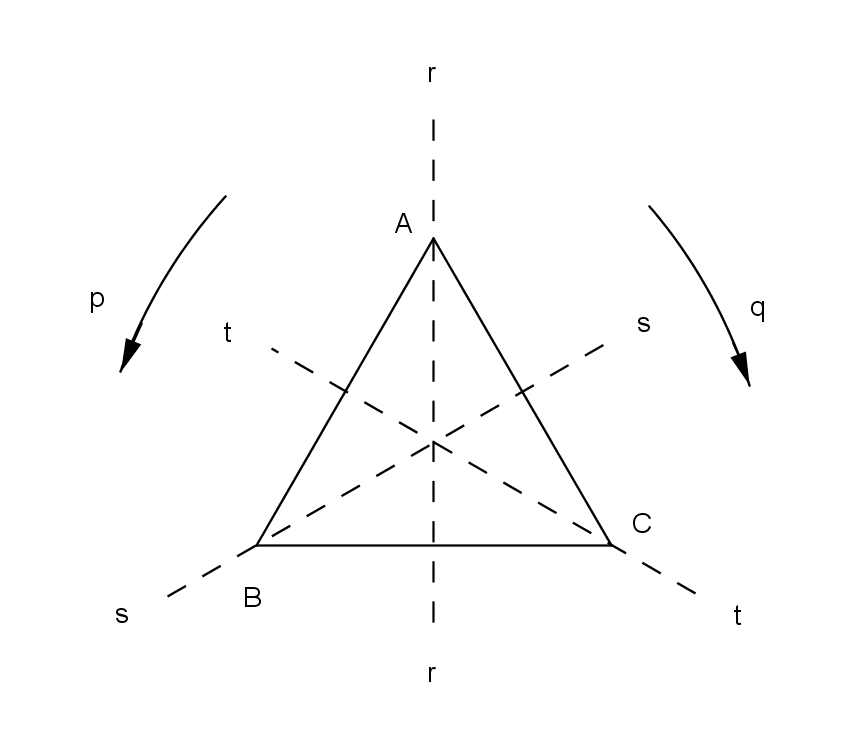
\includegraphics[width=0.5\textwidth]{SymmetryGroupEqTriangle.png}
\end{figure}

Here are the multiplication tables of these two groups.\\

\begin{table}[!htb]
    \begin{subtable}{.4\textwidth}
      \centering
$\begin{array}{c|cccccc}
  & e & p & q & r & s & t \\
\hline
e & e & p & q & r & s & t \\
p & p & q & e & s & t & r \\
q & q & e & p & t & r & s \\
r & r & t & s & e & q & p \\
s & s & r & t & p & e & q \\
t & t & s & r & q & p & e \\
\end{array}$
\caption{Multiplication table for $D_{2n}$}
    \end{subtable}
    \begin{subtable}{.6\textwidth}
      \centering
$\begin{array}{c|cccccc}
  & e & (123) & (132) & (23) & (13) & (12) \\
\hline
e & e & (123) & (132) & (23) & (13) & (12) \\
(123) & (123) & (132) & e & (13) & (12) & (23) \\
(132) & (132) & e & (123) & (12) & (23) & (13) \\
(23) & (23) & (12) & (13) & e & (132) & (123) \\
(13) & (13) & (23) & (12) & (123) & e & (132) \\
(12) & (12) & (13) & (23) & (132) & (123) & e \\
\end{array}$
\caption{Multiplication table for $S_3$}
    \end{subtable} 
\end{table}

One can see that the multiplication tables are of the same form, so there must exist an isomorphism between the two groups.

However, in the case where $n = 12$, we cannot form an isomorphism between the two groups. When $n > 3$, the vertices of the permuted $n$-gon must maintain their edge structure. That is, under any operation adjacent vertices must remain adjacent. There is no way to permute two connected vertices without breaking this adjacency property. So, there exist permutations with no analogue in the dihedral group. Therefore, there can be no isomorphism.

The special case where $n = 3$ does allow arbitrary permutations because every vertex is connected to every other vertex.


\section{Abelian Group Power Homomorphisms}
We first have that $e^k = e$ for all $k$, so identity is preserved. We show the other two properties:
\begin{align*}
f(ab)  &= f(a)f(b) & f(a\inv)  &= f(a)\inv\\
(ab)^k &= a^kb^k   & (a\inv)^k &= (a^k)\inv\\
a^kb^k &= a^kb^k   & (a^k)\inv &= (a^k)\inv
\end{align*}


\section{Odd Numbers in an Even Group}
We first have that $\ord(e) = 1$, so there are $2k - 1$ possible elements with order 2. We first lat some element $a$ have order 2. Then we have that $aa = e \implies a = a\inv$. We know that there are $2k - 1$ possible elements with this property. For every $b$ such that $b \neq b\inv$, we can remove both $b$ and $b\inv$ from the set of possibilities. From the property of unique inverses, we have that finding any such $b$ implies removing exactly two elements from our set of possibilities. This leaves us with an odd number of elements with order 2.

\section{Morphisms Under Composition}
We will denote each $f$ by the tuple $(a,b,c,d)$. First, we see that $e = (1, 0, 0, 1)$ is the identity element. We consider morphisms $f = (a,b,c,d)$ and $g = (i,j,k,l)$. We have
\begin{align*}
f \circ g   = \frac{a(\frac{iz + j}{kz + l}) + b}{c(\frac{iz + j}{kz + l}) + d}
            = \frac{\frac{aiz + aj}{kz + l} + b}{\frac{ciz + cj}{kz + l} + d}
            = \frac{\frac{aiz + aj + bkz + bl}{kz + l}}{\frac{ciz + cj +dkz + dl}{kz + l}}\\
= \frac{aiz + aj + bkz + bl}{ciz + cj + dkz + dl}
= \frac{(ai + bk)z + (aj + bl)}{(ci +dk)z + (cj + dl)}
\end{align*}
So $FL$ is closed under composition. We are given that $ad - bc \neq 0$, so we have that for any $f = (a,b,c,d)$, $f\inv = \frac{(d,-c,-b, a)}{ad - bc}$. 

We see that the given $g(\frac{az + b}{cz + d}) = \begin{bmatrix} a & b\\ c & d \end{bmatrix}$ is a group homomorphism. The identity element $e = (1,0,0,1)$ maps to the identity matrix $\begin{bmatrix} 1 & 0\\ 0 & 1 \end{bmatrix}$. We also have that $f \circ h$ maps to $\begin{bmatrix} a & b\\ c & d \end{bmatrix}\begin{bmatrix} i & j\\ k & l \end{bmatrix} = \begin{bmatrix} ai + bk & aj + bl\\ ci + dk & cj + dl \end{bmatrix}$, so $g(f \circ h) = g(f)g(h)$. Finally, as we showed above, $f\inv$ maps to $g(f)\inv$.

\section{Finite Order Subgroup}
First, $\ord(e) = 1$, so $e \in H$. For any $a$ in $H$, we have that for some $k$, $a^k = e$. We have
\begin{align*}
a^k &= e\\
(a\inv)^k a^k &= (a\inv)^k\\
e &= (a\inv)^k
\end{align*}
So if $a$ is in $H$, $a\inv$ is also in $H$. It is easy to show that if $a^k = e$, then $a^{nk} = e$. Given $a^m = e$ and $b^n = e$, we can use that fact to show that $ab$ is in $H$. Let $l$ be the least common multiple of $n$ and $m$. Because $l$ is a multiple of both $n$ and $m$, we have that $(ab)^l = a^{cm}b^{dn}$ where $cm = dn = l$. So $(ab)^l = e^2 = e$ and $ab$ is in $H$.


\section{Normal Subgroup Generated by Commutators}
Given $g$ in $G$ and $h$ in $H$, we have
\[
g h g\inv = (g h g\inv h \inv) h = [g, h] h
\]

As $g h g\inv$ can be expressed as a product of commutators, we have that $g h g\inv$ is in $H$, and $H$ is therefore a normal subgroup.

\section{Centralizer Subgroup}
First, we have that the identity element $e$ is in $C_G(x)$, as $ex = xe$. Next, for $a,b$ in $C_G(x)$ we have
\begin{align*}
(ab)x &= x(ab) & a\inv x &= x a\inv\\
a(bx) &= (xa)b & x &= (a x) a\inv\\
a(xb) &= (xa)b & x &= (x a) a\inv\\
(ax)b &= (ax)b & x a &= x a
\end{align*}
So the group is closed and contains inverses for every element. Therefore $C_G(x)$ is a subgroup.



\end{document}
